\documentclass[aspectratio=169, 10pt]{beamer}

\usetheme{Madrid}
\usecolortheme{whale}
\setbeamertemplate{navigation symbols}{}
\setbeamertemplate{footline}[frame number]

\definecolor{meteoblue}{RGB}{0,82,147}
\definecolor{meteoaccent}{RGB}{255,140,0}
\definecolor{lightgray}{RGB}{245,245,245}
\definecolor{darkgreen}{RGB}{0,120,60}

\setbeamercolor{frametitle}{bg=meteoblue, fg=white}
\setbeamercolor{title}{bg=meteoblue, fg=white}
\setbeamercolor{structure}{fg=meteoblue}
\setbeamercolor{block title}{bg=meteoblue!80, fg=white}
\setbeamercolor{block body}{bg=lightgray}
\setbeamercolor{alerted text}{fg=meteoaccent}
\setbeamercolor{block title alerted}{bg=meteoaccent!90, fg=white}
\setbeamercolor{block title example}{bg=darkgreen!80, fg=white}
\setbeamercolor{block body example}{bg=darkgreen!8}

\usepackage[utf8]{inputenc}
\usepackage[T1]{fontenc}
\usepackage{amsmath, amssymb}
\usepackage{booktabs}
\usepackage{graphicx}
\usepackage{xcolor}
\usepackage{tikz}
\usepackage{pgfplots}
\pgfplotsset{compat=1.18}

\title[Data Battle 2026 -- Meteorage]{%
  \textbf{Prediction Probabiliste de la Fin d'Alerte Foudre}\\[4pt]
  \large Processus de Hawkes, LightGBM \& Quantile Regression}
\subtitle{Data Battle 2026 -- Meteorage}
\author{ZEROUALI Mohammed Amine \& BOUBEKRI Saad}
\date{Mars 2026}
\institute{Equipe L2ay2ay}

\begin{document}

%% ── Titre ────────────────────────────────────────────────────────────────────
\begin{frame}[plain]
  \begin{tikzpicture}[remember picture, overlay]
    \fill[meteoblue] (current page.north west) rectangle ([yshift=-1.8cm] current page.north east);
    \fill[meteoaccent!80] (current page.south west) rectangle ([yshift=0.6cm] current page.south east);
  \end{tikzpicture}
  \vspace{1.2cm}
  \titlepage
\end{frame}

%% ── Plan ─────────────────────────────────────────────────────────────────────
\begin{frame}{Plan}
  \tableofcontents[hideallsubsections]
\end{frame}

%% =============================================================================
\section{Probleme et donnees}
%% =============================================================================

\begin{frame}{Probleme, donnees et objectif}
  \begin{columns}[T]
    \column{0.48\textwidth}
      \begin{block}{Contexte}
        \begin{itemize}
          \item Activites au sol suspendues des qu'un impact survient dans \textbf{20 km} d'un aeroport
          \item Regle actuelle : \textbf{30 min fixes} apres le dernier impact, quelle que soit la dynamique de l'orage
          \item \textbf{Chaque minute compte} -- chargement, maintenance, embarquement
        \end{itemize}
      \end{block}
      \vspace{0.2cm}
      \begin{alertblock}{Objectif}
        Calculer a chaque instant $\tau_n$ le delai minimal $u^*$ tel que : P \!\left(T > \tau_n + u^* \mid \mathcal{H}_n\right) < \varepsilon \\
        \textbf{Gain} $= 30 - u^*$ min. Contrainte jury : risque $R < 2\%$.
      \end{alertblock}

    \column{0.49\textwidth}
      \begin{block}{Donnees Meteorage (10 ans)}
        \begin{itemize}
          \item 230\,000 impacts de foudre
          \item 6 aeroports europeens
          \item Localisation + horodatage millimetre
          \item Zone alerte : 20 km | Zone etendue : 50 km
        \end{itemize}
      \end{block}
      \vspace{0.2cm}
      \begin{block}{Notre approche hybride}
        \centering
        \small
        \begin{tabular}{cc}
          \toprule
          \textbf{Hawkes (MLE)} & \textbf{LightGBM} \\
          \midrule
          Modele generatif & Modele supervisé \\
          Interpretable & Non-linearites \\
          $\lambda^*(\tau_n)$ en feature & 13 quantiles \\
          \midrule
          \multicolumn{2}{c}{\textbf{Hybride :} $\lambda^*(\tau_n) \in f_n$} \\
          \bottomrule
        \end{tabular}
      \end{block}
  \end{columns}
\end{frame}

%% =============================================================================
\section{Pretraitement}
%% =============================================================================

\begin{frame}{Pretraitement -- la deduplication, une etape critique}
  \begin{columns}[T]
    \column{0.50\textwidth}
      \begin{alertblock}{Probleme : multi-detections capteurs}
        Le meme eclair physique est detecte simultanement par plusieurs capteurs
        $\Rightarrow$ doublons qui faussent le MLE.
      \end{alertblock}
      \vspace{0.2cm}
      \begin{block}{Impact quantitatif sur $\hat\alpha$ (Ajaccio)}
        \centering
        \begin{tabular}{lcc}
          \toprule
          Seuil dedup & $\hat\alpha$ & Physique ? \\
          \midrule
          Aucun       & 254.1 imp/min & Non \\
          \textbf{10 sec} & \textbf{0.212 imp/min} & \textbf{Oui} \\
          1 min       &   0.049 imp/min & Non \\
          \bottomrule
        \end{tabular}
      \end{block}

    \column{0.47\textwidth}
      \begin{block}{Pipeline de pretraitement (5 etapes)}
        \begin{enumerate}
          \item Parsing UTC $\to$ minutes Unix
          \item Filtrage dist $\leq$ 20 km (alerte) et $\leq$ 50 km (features spatiales)
          \item \textbf{Deduplication a 10 secondes} par aeroport
          \item Segmentation par silence de \textbf{30 min}
          \item Timestamps relatifs \emph{et} absolus en parallele
        \end{enumerate}
      \end{block}
      \vspace{0.2cm}
      \begin{exampleblock}{Resultat}
        \begin{itemize}
          \item 2\,113 alertes d'entrainement
          \item 92\,377 points de features
          \item 412 alertes de test couvertes
        \end{itemize}
      \end{exampleblock}
  \end{columns}
\end{frame}

%% =============================================================================
\section{Modele de Hawkes}
%% =============================================================================

\begin{frame}{Pourquoi un processus de Hawkes ?}
  \begin{columns}[T]
    \column{0.50\textwidth}
      \begin{block}{Observation physique}
        \begin{itemize}
          \item Les impacts de foudre \textbf{ne sont pas independants}
          \item Un impact augmente la probabilite d'impacts futurs (\emph{orage actif})
          \item L'effet \textbf{decroit avec le temps} -- orage qui s'eteint
        \end{itemize}
      \end{block}
      \vspace{0.3cm}
      \begin{alertblock}{Modele naturel : auto-excitation}
        
          \lambda^*(t) = \underbrace{\mu}_{\text{fond}}
          + \underbrace{\alpha \sum_{\tau_i < t} e^{-\beta(t-\tau_i)}}_{\text{excitation passee}}
        
        \begin{itemize}
          \item $\lambda^*(t)$ eleve $\Rightarrow$ orage actif
          \item $\lambda^*(t)$ faible $\Rightarrow$ orage en extinction
        \end{itemize}
      \end{alertblock}

    \column{0.47\textwidth}
      \begin{block}{De $\lambda^*$ a $u^*$}
        La probabilite d'aucun nouvel impact sur $[\tau_n, \tau_n + u]$ :
        \[
          P\!\left(T > \tau_n + u \mid \mathcal{H}_n\right)
          = \exp\!\left(-\int_{\tau_n}^{\tau_n+u} \lambda^*(s)\,\mathrm{d}s\right)
        \]
        On cherche :
        \[
          u^* = \inf\!\left\{u \in [0,30] \;\Big|\;
          P(T > \tau_n + u \mid \mathcal{H}_n) < \varepsilon \right\}
        \]
      \end{block}
      \vspace{0.2cm}
      \begin{exampleblock}{Role cle pour LightGBM}
        $\lambda^*(\tau_n)$ est la \textbf{2\textsuperscript{e} feature la plus importante}
        du modele LightGBM -- lien direct entre physique et prediction.
      \end{exampleblock}
  \end{columns}
\end{frame}

\begin{frame}{Parametres Hawkes par aeroport et limites du modele}
  \begin{columns}[T]
    \column{0.50\textwidth}
      \begin{block}{Parametres MLE (methode d'Ogata)}
        \centering
        \footnotesize
        \begin{tabular}{lcccc}
          \toprule
          & $\hat\mu$ & $\hat\alpha$ & $\hat\beta$ & $\hat\alpha/\hat\beta$ \\
          \midrule
          Ajaccio  & 0.056 & 0.212 & 0.241 & 0.880 \\
          Bastia   & 0.056 & 0.215 & 0.237 & 0.904 \\
          Biarritz & 0.054 & 0.231 & 0.253 & 0.914 \\
          Nantes   & 0.057 & 0.231 & 0.256 & 0.903 \\
          Pise     & 0.056 & 0.204 & 0.229 & 0.892 \\
          \bottomrule
        \end{tabular}
        \vspace{0.1cm}

        Ratio $\hat\alpha/\hat\beta < 1$ : stationnarite garantie.\\
        Variations faibles entre aeroports : dynamique universelle.
      \end{block}

    \column{0.47\textwidth}
      \begin{alertblock}{Limite identifiee : $\mu$ constant}
        Test KS rejete ($p < 0.001$, KS $\approx 0.28$--$0.38$).\\[4pt]
        Cause : $\mu = \text{const}$ ne capte pas le cycle de vie fini
        de l'orage. Le modele simule des alertes trop longues
        ($\approx 160$ min vs $60$--$140$ min observees).
      \end{alertblock}
      \vspace{0.2cm}
      \begin{exampleblock}{Ce que Hawkes apporte malgre tout}
        $\lambda^*(\tau_n)$ reste une \textbf{feature hybride cle} :\\[3pt]
        valeur elevee $\Rightarrow$ orage actif,\\
        valeur faible $\Rightarrow$ orage qui se calme.\\[3pt]
        $\Rightarrow$ Capturee et exploitee par LightGBM.
      \end{exampleblock}
  \end{columns}
\end{frame}

%% =============================================================================
\section{LightGBM Quantile}
%% =============================================================================

\begin{frame}{LightGBM -- Quantile regression et courbe de survie}
  \begin{columns}[T]
    \column{0.45\textwidth}
      \begin{block}{Approche}
        Cible : $y = \tau_{n+1} - \tau_n \in (0, 30]$ min\\[5pt]
        13 modeles (pinball loss) pour $q \in \{5\%, \ldots, 95\%\}$\\[5pt]
        $\Rightarrow$ CDF empirique $\hat{F}_{Y|f_n}$\\
        $\Rightarrow$ courbe de survie $\hat{S}(u) = 1 - \hat{F}(u)$\\
        $\Rightarrow$ $u^* = \inf\{u \mid \hat{S}(u) < \varepsilon\}$
      \end{block}
      \vspace{0.15cm}
      \begin{block}{Vecteur $f_n \in \mathbb{R}^{12}$}
        \footnotesize
        \textbf{Top features (gain LightGBM) :}
        \begin{enumerate}
          \item \texttt{ia\_mean5} -- moyenne 5 dernieres inter-arrivees
          \item \texttt{lambda\_hawkes} -- intensite Hawkes $\lambda^*(\tau_n)$
          \item \texttt{ia\_mean3} -- fenetre courte de ralentissement
          \item \texttt{amp\_last}, \texttt{prop\_cloud} -- marques meteo
        \end{enumerate}
      \end{block}

    \column{0.52\textwidth}
      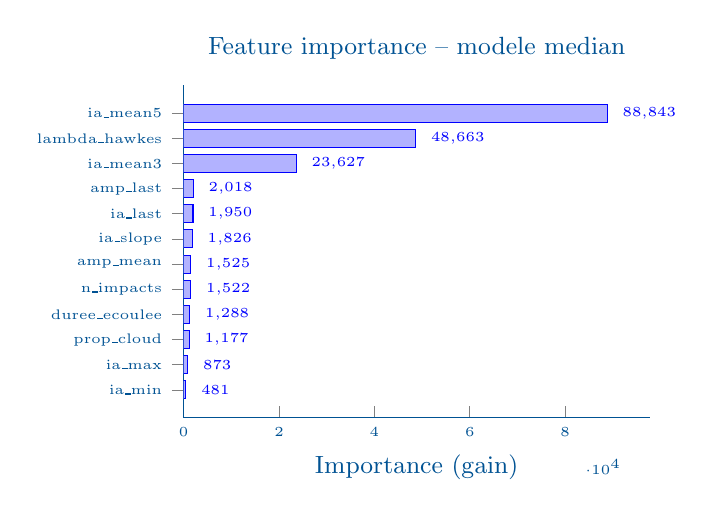
\begin{tikzpicture}
        \begin{axis}[
          xbar, xmin=0,
          width=7.5cm, height=5.8cm,
          bar width=6.5pt,
          ytick=data,
          symbolic y coords={ia\_min, ia\_max, prop\_cloud, duree\_ecoulee,
                             n\_impacts, amp\_mean, ia\_slope, ia\_last,
                             amp\_last, ia\_mean3, lambda\_hawkes, ia\_mean5},
          axis x line*=bottom, axis y line*=left,
          xlabel={\small Importance (gain)},
          xtick={0,20000,40000,60000,80000},
          xticklabel style={font=\tiny},
          yticklabel style={font=\tiny},
          nodes near coords={\pgfmathprintnumber[fixed,precision=0]{\pgfplotspointmeta}},
          nodes near coords style={font=\tiny, xshift=2pt},
          color=meteoblue, fill=meteoblue!60,
          title={\small Feature importance -- modele median},
          title style={font=\small},
          ]
          \addplot coordinates {
            (481,ia\_min)(873,ia\_max)(1177,prop\_cloud)
            (1288,duree\_ecoulee)(1522,n\_impacts)(1525,amp\_mean)
            (1826,ia\_slope)(1950,ia\_last)(2018,amp\_last)
            (23627,ia\_mean3)(48663,lambda\_hawkes)(88843,ia\_mean5)
          };
        \end{axis}
      \end{tikzpicture}
  \end{columns}
\end{frame}

%% =============================================================================
\section{Resultats}
%% =============================================================================

\begin{frame}{Gain vs Risque -- courbe de Pareto}
  \begin{center}
    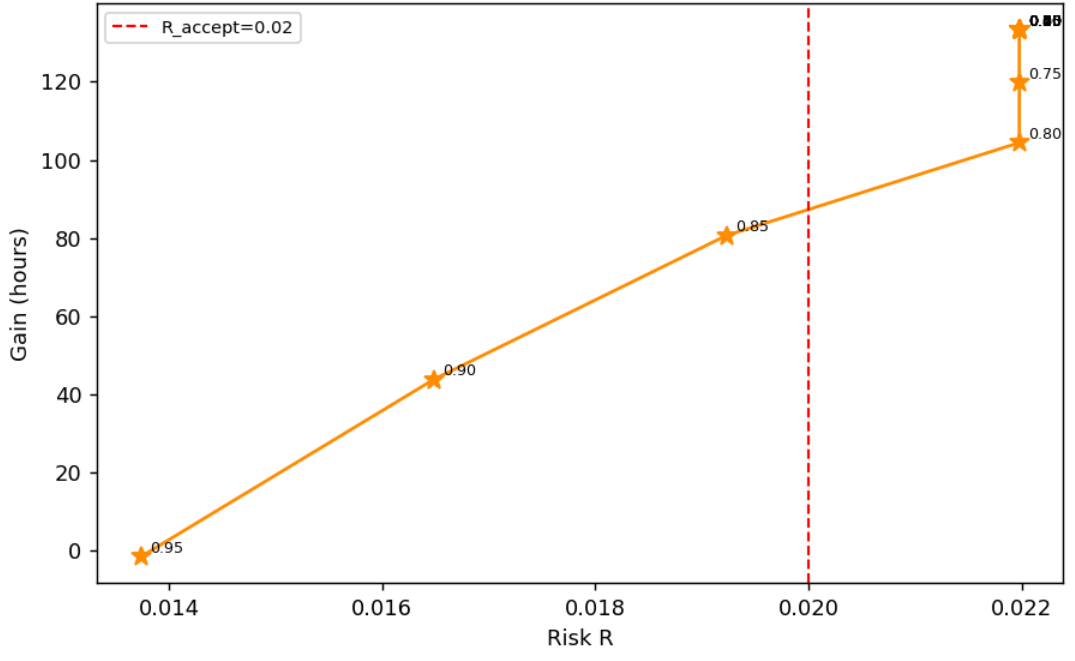
\includegraphics[width=0.7\linewidth]{evaluation_results.png}
  \end{center}
  \vspace{-0.2cm}
  \begin{center}
    \small La courbe doit etre lue du \textbf{coin superieur gauche} (fort gain, faible risque).
    Le seuil $\theta^* = 0.85$ est le meilleur point respectant $R < 2\%$.
  \end{center}
\end{frame}

\begin{frame}{Resultats finaux -- evaluation jury}
  \begin{columns}[T]
    \column{0.50\textwidth}
      \begin{alertblock}{Resultat cle ($\theta^* = 0.85$)}
        \centering\large
        \textbf{80 heures gagnees}\\[4pt]
        \normalsize Risque $R = 1.82\% < 2\%$ \checkmark
      \end{alertblock}
      \vspace{0.2cm}
      \begin{block}{Detail par aeroport}
        \footnotesize
        \centering
        \begin{tabular}{lrrc}
          \toprule
          Aeroport & Alertes & Gain (h) & Manques \\
          \midrule
          Ajaccio  &  96 & 25.5 & 2 \\
          Bastia   & 141 & 20.3 & 5 \\
          Biarritz & 118 &  7.8 & 0 \\
          Nantes   &  45 &  5.7 & 0 \\
          Pise     & 146 & 21.3 & 0 \\
          \midrule
          \textbf{Total} & \textbf{546} & \textbf{80.6} & \textbf{7} \\
          \bottomrule
        \end{tabular}
      \end{block}

    \column{0.47\textwidth}
      \begin{block}{Chiffres cles du pipeline}
        \footnotesize
        \begin{tabular}{lc}
          \toprule
          Donnees d'entrainement & 92\,377 exemples \\
          Modeles entraines & 13 quantiles \\
          Alertes test couvertes & 412 / 612 \\
          Predictions generees & 323\,820 lignes \\
          \midrule
          Seuil optimal $\theta^*$ & 0.85 \\
          Risque $R$ & 1.82\% \\
          Gain total & 80 heures \\
          Temps entrainement & $<$ 5 min CPU \\
          \bottomrule
        \end{tabular}
      \end{block}
      \vspace{0.2cm}
      \begin{exampleblock}{Calibration des quantiles}
        Couverture reelle $\approx$ quantile theorique :\\
        ex. $q = 0.80 \to 79.9\%$ observes.\\
        $\Rightarrow$ Le modele est \textbf{bien calibre}.
      \end{exampleblock}
  \end{columns}
\end{frame}

%% =============================================================================
\section{Responsabilite et impact}
%% =============================================================================

\begin{frame}{Sobriete numerique et impact metier}
  \begin{columns}[T]
    \column{0.48\textwidth}
      \begin{exampleblock}{Green coding}
        \begin{itemize}
          \item \textbf{100\% local} : aucun GPU, aucun cloud
          \item Entrainement LightGBM (92\,000 ex., 13 modeles) : \textbf{$<$ 5 min CPU}
          \item Inference vectorisee : 37\,000 predictions en \textbf{$<$ 30 s}
          \item Empreinte memoire : $<$ 500 Mo RAM
        \end{itemize}
      \end{exampleblock}
      \vspace{0.2cm}
      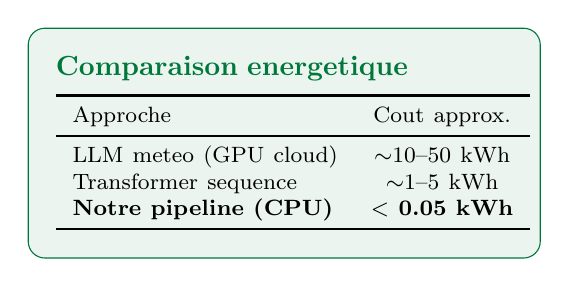
\begin{tikzpicture}
        \node[draw=darkgreen, rounded corners=6pt, fill=darkgreen!8,
              text width=5.8cm, inner sep=10pt]{
          \textbf{\textcolor{darkgreen}{Comparaison energetique}}\\[4pt]
          \footnotesize
          \begin{tabular}{lc}
            \toprule
            Approche & Cout approx. \\
            \midrule
            LLM meteo (GPU cloud) & $\sim$10--50 kWh \\
            Transformer sequence  & $\sim$1--5 kWh \\
            \textbf{Notre pipeline (CPU)} & \textbf{$<$ 0.05 kWh} \\
            \bottomrule
          \end{tabular}
        };
      \end{tikzpicture}

    \column{0.49\textwidth}
      \begin{block}{Impact operationnel}
        \begin{itemize}
          \item \textbf{80 heures} gagnees sur 412 alertes test
          \item Reprise plus rapide : chargement, maintenance, embarquement
          \item Risque residuel $\varepsilon$ explicite -- outil de decision pour les responsables securite
        \end{itemize}
      \end{block}
      \vspace{0.2cm}
      \begin{block}{Extensions futures}
        \begin{itemize}
          \item \textbf{Hawkes marque} : $\alpha(d_i)$ integrant dist/amp
          \item \textbf{Hawkes non stationnaire} : $\mu(t)$ pour le cycle de vie de l'orage
          \item \textbf{API FastAPI} : flux Meteorage en temps reel
          \item \textbf{Quantile conforme} pour garanties exactes de couverture
        \end{itemize}
      \end{block}
  \end{columns}
\end{frame}

%% ── Merci ─────────────────────────────────────────────────────────────────────
\begin{frame}[plain]
  \begin{tikzpicture}[remember picture, overlay]
    \fill[meteoblue] (current page.south west) rectangle ([yshift=2cm] current page.south east);
  \end{tikzpicture}
  \vspace{1.4cm}
  \begin{center}
    {\Large \textbf{Merci pour votre attention !}}\\[0.7cm]
    {\large Questions ?}\\[0.8cm]
    \small Code source disponible sur GitHub -- equipe L2ay2ay
  \end{center}
\end{frame}

\end{document}